\documentclass{beamer}

% Top-aligning columns within a top-aligned frame
% https://tex.stackexchange.com/questions/16447/beamer-top-aligning-columns-within-a-top-aligned-frame
\makeatletter
\newenvironment{myitemize}{%
   \setlength{\topsep}{0pt}
   \setlength{\partopsep}{0pt}
   \renewcommand*{\@listi}{\leftmargin\leftmargini \parsep\z@ \topsep\z@ \itemsep\z@}
   \let\@listI\@listi
   \itemize
}{\enditemize}
\makeatother  

\usepackage[USenglish]{babel}
\usepackage[utf8]{inputenc}
\usepackage{amssymb, amsmath}
\usepackage{bm}
\usepackage{color}
\usepackage{tikz}
\usepackage{url}

\definecolor{links}{HTML}{2A1B81}
\hypersetup{colorlinks,linkcolor=,urlcolor=links}

\usetheme{Boadilla}
\setbeamertemplate{headline}{}
\newcommand*\oldmacro{}%
\let\oldmacro\insertshorttitle%
\renewcommand*\insertshorttitle{%
  \oldmacro\hfill%
  \insertframenumber\,/\,\inserttotalframenumber}
  

\bibliographystyle{apalike}
% make bibliography entries smaller
%\renewcommand\bibfont{\scriptsize}
% Now get rid of all the colours
\setbeamercolor*{bibliography entry title}{fg=black}
\setbeamercolor*{bibliography entry author}{fg=black}
\setbeamercolor*{bibliography entry location}{fg=black}
\setbeamercolor*{bibliography entry note}{fg=black}

\newcommand{\lnorm}[1]{\left\lVert#1\right\rVert^2}
\newcommand{\norm}[1]{\left\lVert#1\right\rVert}

% and kill the abominable icon
\setbeamertemplate{bibliography item}{}

\begin{document}
\title{Dropout is a special case of the stochastic delta rule: faster and more accurate
deep learning}  
\author{Radek Bartyzal}
\date{28. 2. 2019} 
\institute{Let's talk ML in Prague}

\frame{\titlepage} 

\begin{frame}{Dropout}

\begin{itemize}
\item add stochasticity = escape local minima
\item removes hidden units according to a Bernoulli
random variable with probability p prior to each
update

\item $\implies$ gradient updates affect non-removed neurons only
\item $\implies$ exponential number of networks averaged over updates
\item $\implies$ increase generalization by model averaging
\end{itemize}

\end{frame}
%--------- END Frame 1 -------------
\begin{frame}{Stochastic Delta Rule}

\begin{itemize}
\item each weight $w_{ij}$ = random variable with mean $\mu_{w_{ij}}$ and standard
deviation $\sigma_{w_{ij}}$
\item weight random variable is
sampled on each forward activation
\item $\implies$ exponential number of potential networks with shared weights
\item Both parameters are
updated according to prediction error
\item $\implies$ weight noise injections reflecting local history of prediction error and local model averaging
\item $\implies$ simulated annealing per weight
\end{itemize}

\end{frame}
%--------- END Frame 1 -------------
\begin{frame}{Stochastic Delta Rule}

\begin{itemize}
\item 
\end{itemize}

\end{frame}
%--------- END Frame 1 -------------
\begin{frame}{Stochastic Delta Rule}

\begin{itemize}
\item 
\end{itemize}

\end{frame}

%--------- END Frame 7 -------------
\begin{frame}{Results}
\begin{figure}[h]
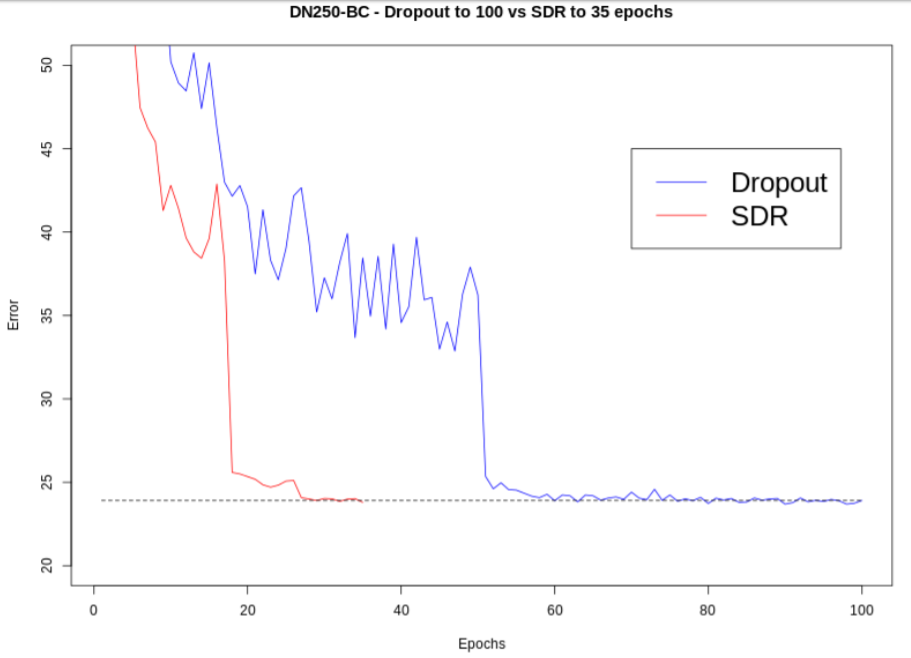
\includegraphics[width=0.9\textwidth]{img/dropout_vs_sdr}
\end{figure}
\end{frame}
%--------- END Frame 7 -------------
\begin{frame}{Results}
\begin{figure}[h]
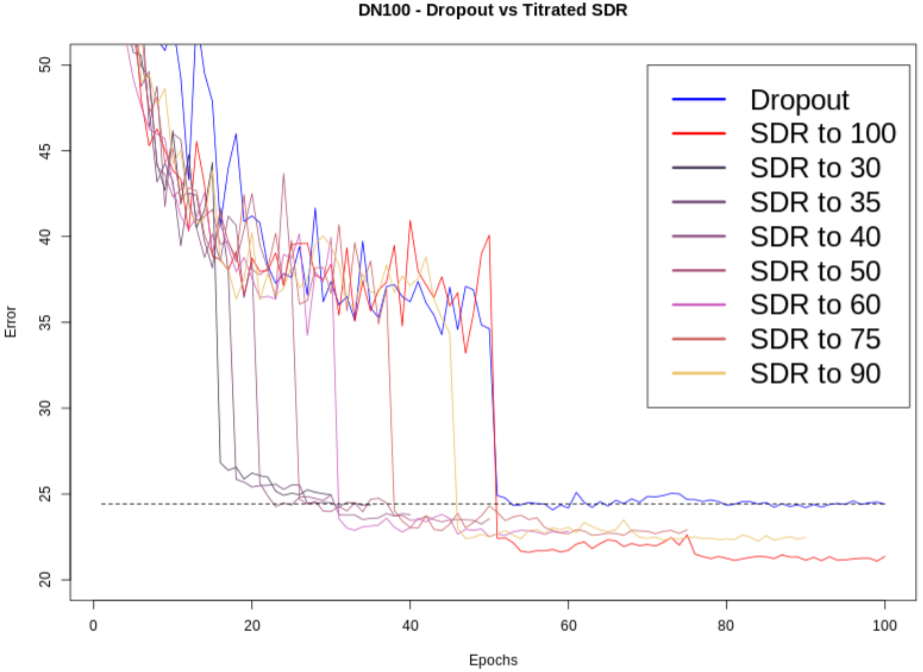
\includegraphics[width=0.9\textwidth]{img/titrated}
\end{figure}
\end{frame}

%--------- END Frame 12 -------------
\begin{frame}{Sources}

\begin{thebibliography}{0}

  \bibitem[1]{cit:drop} 1. Frazier-Logue, Noah, and Stephen José Hanson. "Dropout is a special case of the stochastic delta rule: faster and more accurate deep learning." arXiv preprint arXiv:1808.03578 (2018). \url{https://arxiv.org/pdf/1808.03578v2.pdf}
  
\end{thebibliography}

\end{frame}

 
 
 
\end{document}
